\documentclass[paper=a4, fontsize=10pt]{report}

\usepackage[english]{babel}
\newcommand{\sql}{\textbf{SQL}}	
\usepackage{listings}
\renewcommand{\lstlistingname}{Code Example}% Listing -> Algorithm
\usepackage{booktabs}
\usepackage[utf8x]{inputenc}
\usepackage{lmodern,textcomp}

		% English language/hyphenation	
\usepackage{amsmath,amsfonts,amsthm} % Math packages
\usepackage[pdftex]{graphicx}	
\usepackage{url}

\title{Small Exercise}
\author{Pietro della Briotta Parolo}
\date{}


%%% Begin document
\begin{document}
\maketitle
\section*{Data Processing}

The first thing I did was to convert the csv data into a sqlite database, which is easier to handle. This was done in python
simply by reading the csv file and adding each row into the newly created \textit{events} table that I had previously created. Furthermore,
I decided to add an index for each \textit{uid} in order to be able to perform user based searches faster.

\section*{Question 1}

\textit{ Calculate the average number of song/minigame\_plays before a user 
subscribes.}

\textbf{3.55 or 4.33 according to whether users who create an account without playing songs or minigames are included.}\\

In order to obtain this result I needed a subscription time stamp for each user that subscribed. This was easily done with an SQL query:


\footnotesize
\begin{lstlisting}[frame=single,caption=Generate subscription table \label{code:sub_table}]
  CREATE TABLE  subscribed  AS
  SELECT uid,date
  FROM events
  WHERE event = 'subscribed'
        
\end{lstlisting} 
\normalsize

This allows me to have a time stamp to be used in order to check which uid events took place before the user subscribed. The next step therefore was to return the number of pre-subscription events.

\footnotesize
\begin{lstlisting}[frame=single,caption=Return pre-sub events \label{code:pre_sub_table}]
 SELECT COUNT(*) 
 FROM subscribed 
 LEFT JOIN events
 USING (uid)
 WHERE events.date < subscribed.date
 AND  event in ('minigame_played','song_played')
\end{lstlisting}
\normalsize

The script returns 2146 events, which divided by the number of subscriptions (605) gives me
\textbf{3.55} songs or minigames on average before subscription.

A more elegant and direct way to solve the issue is to use SQL directly. This can be achieved by
counting the events for each uid and then averaging.

\footnotesize
\begin{lstlisting}[frame=single,caption=Return SQL average \label{code:sql_average_table}]
 SELECT AVG(cnt)
 FROM (  
 SELECT count(*) AS cnt
 FROM subscribed 
 LEFT JOIN events USING (uid)
 WHERE (events.date < subscribed.date)
 AND event in ('minigame_played','song_played') 
 GROUP BY (uid)
 )
\end{lstlisting}
\normalsize

The result, for this implementation is different: \textbf{4.33}. This is because in this way of
formulating the query the users who subscribed directly without first playing songs or 
games are not counted in the statistics. In order to obtain the same result as before however, 
one can use a simple trick to force the LEFT JOIN to return at least one event: the subscription event, which can 
later be discarded.

\footnotesize
\begin{lstlisting}[frame=single,caption=Return SQL average - Fixed \label{code:sql_average_fixed_table}]

 SELECT AVG(cnt)
 FROM ( 
 SELECT count(*) -1  AS cnt
 FROM subscribed 
 LEFT JOIN events USING (uid)
 WHERE (events.date <= subscribed.date)
 AND event in ('minigame_played','song_played','subscribed') 
 GROUP BY (uid) )
\end{lstlisting}
\normalsize
This method returns again an average of \textbf{3.55}.


\section*{Question 2}

\textit{Does the group B have a better conversion rate between account created and
the first song played than the control group?}

\textbf{No. Group B has a higher conversion rate, but it is statistically not significant. However, more data could
change the picture.}\\

In order to answer this question I started by doing a similar job as in code example \ref{code:pre_sub_table}, thus creating a table that stores the time stamp
for the account creation. This allows me to check for individual uid activity after account creation. Similarly again, the SQL search is very similar to the 
the previous question, where in this case I filter for \textit{song\_played} events after the account creation.


\footnotesize
\begin{lstlisting}[frame=single,caption=Return conversion rates \label{code:sql_average_fixed_table}]
SELECT COUNT(DISTINCT(uid)) 
FROM account 
LEFT JOIN events USING (uid)
WHERE events.date > account.date
AND event = 'song_played'
AND groupName = a/b
\end{lstlisting}
\normalsize

The query returns 326 and 330 for groups a and b respectively. Both groups have 333 users, thus giving us a very high conversion rate for both groups:
\begin{itemize}
 \item Group A conversion rate: $p_{a} = 0.97898$
 \item Group B conversion rate: $p_{b} = 0.99099$
\end{itemize}


While the numbers are similar, suggesting no significant difference between the two groups, one needs to take into account the sample size and perform
further statistical test.


In this case we want to test the null hypothesis $p_{a} = p_{b}$ which means that both samples are taken from the same binomial distribution having identical
success rate.


From there we can check the null hypothesis by performing a \textit{z test}
\begin{equation}
 z = \frac{p_{a}-p_{b}}{\sqrt{p(1-p)(\frac{1}{n_{a}} + \frac{1}{n_{b}})}}
\end{equation}
where $n_{a} = n_{b} = 333 $ is the sample size for each group and $ p = \frac{n_{a}p_{a} + n_{b}p_{b}}{ (n_{a} + n_{b})}$ is the weighed average of the two rates,
which in this case is just the arithmetic mean since the two sample groups are identical in size: $p = (0.97898 + 0.99099)/2 = 0.9849445
$. The tests returns a z score of 1.27, which gives us a $\approx 10\%$ probability for the results of group B to be generated from a distribution with higher
conversion rate.
While this value is low, it's usually not considered low enough to reach a definite conclusion. A z score of 1.65 would give a 5$\%$ probability,
which is often considered a reliable indicator. In this case the problem seems to lie in the high conversion rate of the control group,
which requires group B to be pretty much "perfect" in its conversion rate.
However, it is important to notice that the previous method is based on the assumption that the binomial distribution can be approximated with a Gaussian one.
Such approximation increases in validity the higher the sample size and the closer the probability is to 1/2. In our case we do have a significant sample size, but the 
high conversion rate limits the validity of the approximation.

Another way to tackle the problem is to take the control group as a reference point to see whether its statistical properties would be
able to justify the performance of group B. This can be simply done with a binomial test, as shown in code example \ref{code:binomial_test}. In this case, 
the probability
of obtaining 330 or more successes with the conversion rate of the control group is $\approx 8\%$, coherently with what discussed before.

\footnotesize
\begin{lstlisting}[frame=single,caption= Binomial Test\label{code:binomial_test}]
scipy.stats.binom_test(330, 333, 326./333, alternative='greater')
0.079568660226078308
\end{lstlisting}
\normalsize

It's also important to note that had the successes been just one more, this binomial test would have shown statistical significance
for the two conversion rates being different. The same would have happened with a sample size of 500 users for group B with the 
same conversion rate.
This means that even though the current data cannot show an out-performance by 
group B, the result is on the "edge" of statistical signficance and further data should be collected in order to have stronger
statistical results.

\section*{Question 3}

\textit{In your opinion, is the experiment of the group C bringing more money to the company? Please explain why.}

\textbf{Yes. More than $60\%$ of the subscribed users in both groups are likely to remain subscribed indefinitely, allowing
the higher weekly cost of group C to counterbalance the higher short-term unsubscription costs of group B.}\\


An initial analysis can be done in a way similar to Question 2 in terms of whether the groups are performing differently in regard to subscription and unsubscription rates.
Table \ref{tab:sub_unsub_rates} shows the numbers of subscribed and unsubscribed users for each group, along with their rates (the unsubscription rates are based on the number of subscribed users, of course).

\begin{table}[htbp]
\normalsize

  \centering
  \caption{Subscriptions and Unsubscriptions for Groups B and C}
    \begin{tabular}{ccccccc}
    \toprule
    \textbf{Group } & \multicolumn{2}{c}{\textbf{Subscribed}} & \multicolumn{2}{c}{\textbf{Unsubscribed}} \\
    \midrule
    B & 199  & 59.76\% & 73  & 36.68\%  \\
    C & 205   & 61.56\% & 76   & 37.07\%  \\
    \bottomrule
    \end{tabular}%
  \label{tab:sub_unsub_rates}%
\end{table}%
\normalsize

With these numbers we can check whether the subscription rates are statistically significantly different.

The z-score for the hypothesis that the two subscription distributions are different is 0.475, implying that there is no significant statistical evidence for one group being more likely to have
subscriptions over the other. The same result applies to the unsubscription rate, which has a z score of 0.145, also revealing no statistical difference.

We can therefore conclude, on a first level of analysis, that the two groups do not appear to perform differently in terms of subscription rates and unsubscription rates. If this 
pattern is confirmed, the difference in revenue for each group ultimately depends on how long the users remain subscribed. In fact, group C has a higher
price on a weekly basis (5,6€ vs 5€), which is
however counterbalanced by the fact that an early unsubscription during the week will be less profitable compared to the unsubscriptions for group B. 
If we assume that there is no preferred day of unsubscription in the 7 days interval, group B will give a $ \frac{\sum_{i=1}^{7} 5-0.8i}{7} =1.8$€ average
extra revenue per user due to the asymmetry in the payments. Given also the 0.6€ weekly extra revenue for group C, we can therefore conclude that if the similarity 
in subscription and
unsubscription rates is confirmed, the daily payment type becomes more profitable only starting from the beginning of the fourth week. 
Is it the case with our data?

This problem is linked to the known problem of \textit{survival analysis}, which aims at estimating "death times" where deaths represent the withdrawal of members from a certain group,
in this case from the subscribed group. In our scenario, we are also facing the issue of censorship, i.e. the presence of users whose death might not have been observed yet. In Fig.\ref{fig:lifetimes} we can see practically what that means: while the red lines show a birth (subscription)
and a death (unsubscription), the blue lines do have a birth but are still missing a death time.
\begin{figure}[h!]
\centering
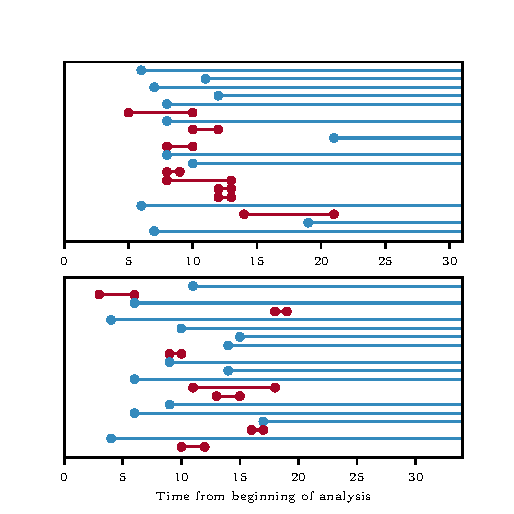
\includegraphics[width=.99\columnwidth]{lifetime.pdf}
\caption{Example of lifetimes for 40 randomly selected users from group B (top) and group C (bottom).}
\label{fig:lifetimes}
\end{figure}

The function that gives the probability of an user to survive time T is called survival function and it can be estimated
with a non-parametric statistic called the Kaplan-Meier estimator, which is defined as:
\begin{equation}
 \hat{S}(T) = \prod_{i: t_{i} < T} \Big(1 - \frac{d_{i}}{n_{i}} \Big)
\end{equation}


What the estimator does is calculate the probability of survival by multiplying the death probabilities in each previous time interval, which
are calculated using the number of deaths $n_{i}$ over the alive population $d_{i}$. The important aspect of this 
estimator is that at the same time it does not require information on the actual functional form of the survival function
and it also allows to approximate its variance. A similarly related concept is the hazard function, which measures
the instantaneous failure rate for a single user: $ \lambda (t) = \frac{-S'(t)}{S(t)}
$. This is in turn allows to calculate the Nelson-Aalen estimator, which estimates the cumulative function of $\lambda(t)$,that
is the sum of all the risk of failure that users have experienced until time T:
\begin{equation}
 \hat{\Lambda}(T) = \prod_{i: t_{i} < T}  \frac{d_{i}}{n_{i}}
\end{equation}



\begin{figure}[h!]
\centering
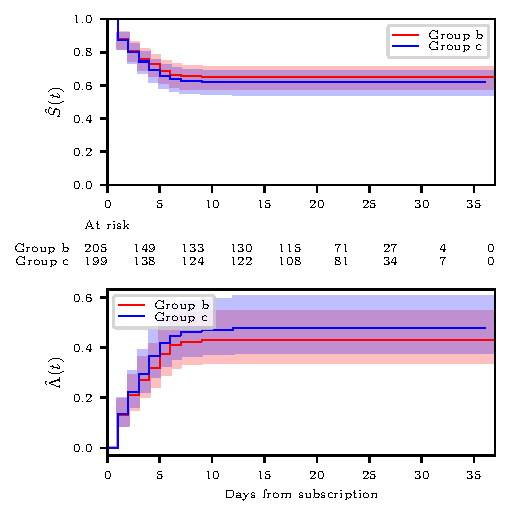
\includegraphics[scale = 0.99]{survival.pdf}
\caption{Survival function (top) and cumulative hazard function (bottom).}
\label{fig:survival}
\end{figure}

Fig.\ref{fig:survival} shows the fitting of both estimators, along with the errors. Both estimators shows that, for both groups,
the curves stabilize after 10/15 days at similar values. The estimators are telling us that the users
either unsubscribe within a limited period of time (roughly 10 days) or else are likely to keep their subscription indefinitely. Statistically
speaking, the absence of deaths in the $t \in [11,36]$ range is a strong indicator that users of both groups are extremely unlikely to randomly
unsubscribe after the first 10 day period. 

In the code example \ref{code:python_logRank} we can also see the result of a statistical test
that compares the survival curves of the two groups, showing that there is no statistical difference between the groups.
\scriptsize
\begin{lstlisting}[frame=single,caption=LogRank test \label{code:python_logRank}]
results = logrank_test(b_life,c_life,b_events,c_events, alpha=.99)
results.print_summary()

Results
   df: 1
   alpha: 0.99
   t 0: -1
   test: logrank
   null distribution: chi squared

    p-value | test statistic |  test result       |  is significant
    0.53285 |         0.389  | Cannot Reject Null |       False       

\end{lstlisting}

\normalsize
To summarize we have seen that:
\begin{itemize}
 \item There is no statistical difference between the subscription and unsubscription rates in the two groups
 \item The profitability of one group over the other depends on how long the users remain within the system
 \item The critical time in which group C statistically is more profitable than group B is of 3 weeks
 \item Users most likely either unsubscribe in the first 10 days or else will remain subscribed indefinitely
\end{itemize}

We can thus conclude that, since the payment option of group C does not influence the subscription/unsubscription dynamics, its
higher weekly cost will eventually make it more profitable.


\end{document}

